\chapter{Applications}

\section{Applications}
In the current age, Sensor fusion are used in the systems which were only found in science fiction books and was just an imagination (e.g. self driving car). It has become the key component for moving object detection and tracking\cite{Cho_2014, Chavez_Garcia_2016}, obstacle detection\cite{Shinzato_2014} which are the most challenging task in the application domain of autonomous driving cars. In the following parts of this paper, some of the successful application of sensor fusion is described.


\section{Multiple Sensor Fusion for Moving Object Detection and Tracking}
The intelligent vehicles are now becoming capable of instruct themselves to drive in very dynamic and unstructured environment. But driving in such an environment increase uncertainty. One of the uncertain task is to moving object detection and tracking. Perceiving the environment involves the selection of different sensors to obtain a detailed description of the environment and an accurate identification of the objects of interest\cite{Chavez_Garcia_2016}. So, Fusion of multiple sensor could decrease the uncertainly in moving object detection task. In the following, two different approaches are described for moving object detection which are different in the view point of the sensors.

\subsection{Front View Approach}
In \cite{Chavez_Garcia_2016}, an advanced driver assistance systems (ADAS) is introduced which main task is to help the drivers to avoid dangerous situations. ADAS assists with warning messages in dangerous driving situations (e.g., possible collisions), activation of safety devices to mitigate imminent collisions, autonomous maneuvers to avoid obstacles, and attention-less driver warnings\cite{Chavez_Garcia_2016}. There are two major tasks to perceive the environment. The task simultaneous localization and mapping (SLAM) is one of and another one is to detect and track the moving objects (DATMO). The model of perception task is shown in figure \ref{fig:datmoslam}.
\begin{figure}
  \centering
  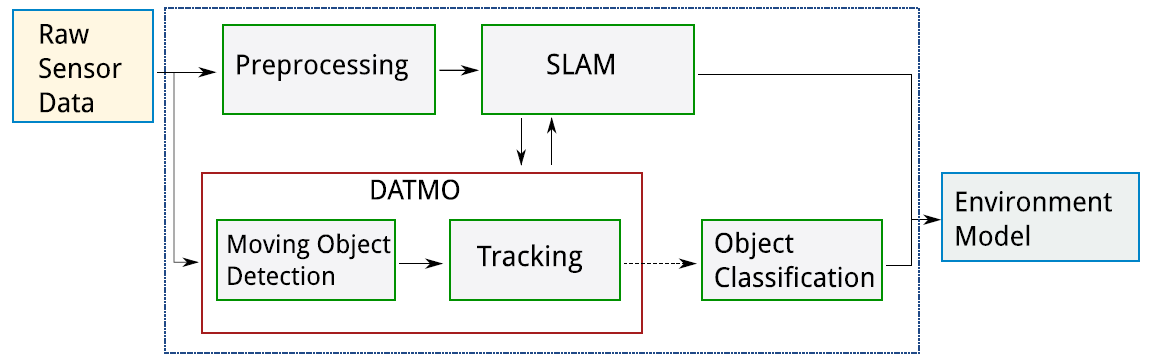
\includegraphics[width=.4\textwidth]{src/pic/datmo_slam_arch.png}
  \caption{General Architecture of perception task. \cite{Chavez_Garcia_2016}}
  \label{fig:datmoslam}
\end{figure}
\begin{description}
    \item[SLAM:] could be defined as follows. A self driving car is moving in an unknown environment and it starts moving from a known location. Meanwhile, it's motion is uncertain which makes the determination of it's global position more difficult. As it is moving, continuously it perceives the environment. In this situation, SLAM is the procedure of building a map of the environment while simultaneously calculating the cars position relative to the map\cite{Thrun2008}. More formally we can say, the SLAM problem asks if it is possible for a autonomous agent to move to an unknown location in an unknown, dynamic or unstructured environment and for the agent to incrementally build a consistent map of this environment while simultaneously determining its location within this map\cite{Bailey:1638022}.
    \item[DATMO:] While SLAM creates a map of static objects including the position of the agent, DATMO uses the map  of static objects generated by SLAM \cite{Azim:6232303} to determine the object to be moving or static\cite{vu2008mapping}. On the other hand, by perform DATMO it is possible to get the position of moving objects around, track them and even predict the future behaviour of those moving objects\cite{vu2008mapping}.
\end{description}

It is assumed that the SLAM is a solved task. As a result it is more reasonable to focus on the DATMO\cite{Chavez_Garcia_2016}. DATMO is performed with an Evidential fusion approach where object classification is the key component. Additionally, Evidential fusion handle uncertainty of sensor detection. Actual goal is to find a list of moving objects with their velocity which should improves the ADAS.

Handling incomplete environment data is one of the important factor of assistance systems which leads to wrong perception. The reasons for incomplete sensor data are already described in the introduction section of this paper. Including incomplete information, there is another problem exists in the tracking process. The tracking process expects that all inputs are moving objects. But in the real world, environment consists of both moving and static objects. So, moving object detection is a very difficult task of moving object tracking system and various number of sensors need to work together to perform the task.

\subsubsection{Motivation}

\subsubsection{Environment Setup}
In the experiment \cite{Chavez_Garcia_2016}, a Lancia Delta car is decorated with necessary equipment such as a processing unit for processing the image and create moving object list, some components which is responsible for driver interaction and the front - facing sensors i.e., Lidar, Camera and Radar. So the sensors only cover the front view of the vehicle as shown in figure \ref{fig:sensorcovarage}. An IBEO Lux laser scanner is used as the lidar sensor which can deliver a 2D list of impact points and it can cover all the points in the range of 200m. The radar is used to detect moving targets. It could detect targets within 150m and the velocity range up to 250kph. The camera would capture black and white images.

\subsubsection{System Architecture}
The fusion process is performed in a Perception System (PS) which is developed according to improve the efficiency and increase the quality of sensor data. It tries to concentrate on object detecting and tracking to improve the data quality. The PS aims at detecting, classifying and tracking a set of moving objects of interest that may appear in front of the vehicle\cite{Chavez_Garcia_2016}. The structure of the  PS is shown in Figure \ref{fig:PS}. In this system, the fusion module is taking input directly from the three sensors. Initially lidar, radar and camera get the input from the environment and create a list of detected objects for each sensor. Those three lists are then provided to the fusion module. Each environment object is demonstrated by their position, size and evidence distribution of class hypotheses. On the other hand, classifications are done by the shape, relative speed and visual appearance of the detected objects. Precisely, the lidar and radar is performing the task of detection while camera is extracting the features of the detected objects to classify them. The fusion module fused the three list of objects and combined them into one list  where each object contains combined description. The ultimate output of the fusion method is provided to the tracking module to calculate the moving objects states which is actually the final output of the DATMO task. Three sensors are contribution in the task of moving object detection and tracking. The next sections are going to describe briefly how the the sensors prove information for detection and tracking.

\begin{figure}
    \centering
    \begin{subfigure}[b]{0.4\textwidth}
        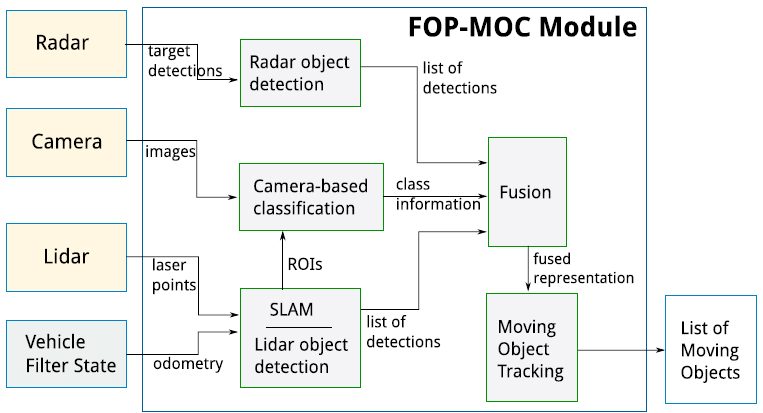
\includegraphics[width=\textwidth]{src/pic/PS.png}
        \caption{}
        \label{fig:PS}
    \end{subfigure}
    \begin{subfigure}[b]{0.4\textwidth}
        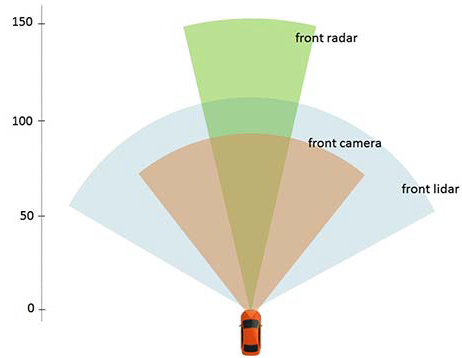
\includegraphics[width=\textwidth]{src/pic/sensor_covarage_front.png}
        \caption{}
        \label{fig:sensorcovarage}
    \end{subfigure}
    \caption{\ref{fig:PS}:Sensor Fusion model, \ref{fig:sensorcovarage}:Coverage of the sensors}
    \label{fig:group1}
\end{figure}

\subsubsection{Moving Object Detection}
The process of three individual sensors for Moving object detection are described bellow:
\begin{description}
    \item[Lidar Processing:] Lidar is used as the leading sensor in the setup as it can produce high resolution data with more accurate result. The principal task of lidar is to get exact information of the shape of the moving object in front of the vehicle. Though the main pourpose is to focus on DATMO task, the SLAM component is also implemented to get the map of objects and vehicles position in the map\cite{Chavez_Garcia_2016}. By the lidar data a 2D Bayesian occupancy grid map is created. Each cell in the map is filled with or not by an object where vehicles location if found by Maximum Likelihood approach. Each time the sensor updates, the map is recalculated and the vehicle position is also re-estimated. Besides, lidar based detection also works with the help of the grid map. If the a cell of grid map is occupied with an obstacle which was previously free cell, then it is said to be a moving object. In the contrast, if a cell is occupied with an object which was also previously occupied, then it is said to be a static object. The SLAM process is completely independent from the moving object detection task.
    \item[Camera Images:] The camera images are processed to extract the visual features and classification.
    \begin{enumerate}
        \item{Visual Representation:} The Histograms of Oriented Gradients (HOG) descriptor is taken as the core of vehicle and pedestrian visual representation as it has already shown promising results\cite{Chavez_Garcia_2016}. The main goal is to extract the graphical details of the particular area of the image which is important to extract for future use to find out the existence of the object of interest. A sparse version of the HOG descriptor (S-HOG) is proposed to use instead of actual HOG descriptor which focuses on specific areas of an image patch \cite{Chavez_Garcia_2016}. S-HOG reduces the common high-dimensional HOG descriptor to explains the selected block of the image of different class.
        \item{Object Classification:} Detecting the region of interest (ROI) from camera image is a performance degrading task. On the other hand, the ROI is already available from lidar sensor and that is why already provided ROI is used in the camera images to specify object region. Every ROI is processed to extract the visual features and a classifier is applied to decide if an object of interest is inside the ROI. As the speed and quality of the result is totally depend on the choice of the classifier, an optimized and boosting-based learning algorithm is implemented which is called discrete Adaboost\cite{Chavez_Garcia_2016}. This algorithm combines many week classifiers and combine them to make the powerful one which increase the performance. For each class of interest e.g., pedestrian, bike, car, truck, a binary classifier was trained off-line to identify object (positive) and non-object (negative) patches\cite{Chavez_Garcia_2016}.
    \end{enumerate}
    \item[Radar Targets:] Radar sensor has a build in method to detect moving objects. Radar creates a list of n moving objects and send the list to perception approach. Each element of the list contains the range, direction of moving and relative speed of the detected target. There are some limitation of Radar sensor. One problem is, Radar also could include static objects in the list. Sometimes the week objects could not always detected by the Radar which leads to miss detection. Because of various problems, the targets are tracked using constant velocity, acceleration and turning models represented by Interactive Multiple Model (IMM).
\end{description}

\subsubsection{Moving Object Classification}
The information about kinetic state of the objects with classification is determined in detection level. The descriptions found from detection level is very useful for better estimation of object's motion and removes number of miss leading detection. In detection level, only one class is selected for the object which means it is not possible to fix the classification if the initial one is wrong. It is necessary to keep more than one approximate classifier so that in case of wrong classification, it is easy to get the correct classifier.

A composite representation is formed by two parts: kinetic + appearance\cite{Chavez_Garcia_2016}. Kinetic description includes position and shape information in a 2D space. Appearance description includes an evidence distribution m($2^{\Omega}$) for all possible class hypothesis where $\Omega$= \{pedestrian, bike, car, truck\} is the frame of discernment representing the classes of interest\cite{Chavez_Garcia_2016}. The fusion module mainly detect and track the objects in the from of $\Omega$ and perform the classification. The process of three individual sensors for Moving object classification are described bellow:
\begin{description}
    \item[Lidar Sensor:] In the detection task, the shape of the moving object is already found. So, the shape of the object can be used for kinetic representation. The modeling of the moving objects are done by a box \{x,y,w,l,c\}, where x and y are the center of the box, w and l are the width and length according to the class of object \cite{Chavez_Garcia_2016}. But if the moving object is very small, the box model doesn't fit. For example pedestrians are not able to modeled by a box rather it is assume to be a 2D object. So for small objects a point model \{x,y,c\} is suited well where x, y are the 2D coordinate of center of the object and c is the class. Classification of objects is done based on the shape and size of the object which follows a fixed fitting-model approach. It is hard to get the exact classification of moving object because the visibility is temporary. For example, if the width of an object in less than a threshold, it is classified as a bike or pedestrian.
    
    In this way, it is necessary to know the threshold for all classes. The thresholds are defined for examining the size of typical passenger cars, trucks and motorbikes sold in Europe\cite{Chavez_Garcia_2016}. In this experiment, instead of keeping only one class decision, a basic belief assignment $m_{1}(A)$ for each $ A \in \Omega $ is defined, which describes an evidence distribution for the class of the moving object detected by lidar\cite{Chavez_Garcia_2016}.
    \item[Camera Sensor:] In the detection phase, lidar provides a set of ROIs which are used to generate hypothesis that the objects are located in the image at the place of the set of ROIs. To verify the hypothesis, off-line classifiers are applied to classify different objects. The camera image classification extracts more information from a ROI by dividing the ROI into several sub regions. After classification of each ROI has done, a belief assignment $m_{c}$ is calculated which represents the evidence distribution for the classes hypotheses\cite{Chavez_Garcia_2016}.
    \item[Radar Sensor:] This sensor is mainly used for moving object detection. But if other sensors can not classify then this sensor tries to classify moving objects. As radar can determine the speed, speed is used for classification. The slowest speed of the vehicle classes is estimated statistically and determine a threshold for each class. That means for cars, trucks, bikes and pedestrians there is a threshold and if the moving object move in a speed of the threshold than the object classified as the corresponding class. Finally, the basic belief assignment is calculated based on the speed classification\cite{Chavez_Garcia_2016}.
\end{description}

\subsubsection{Sensor Fusion}
Once the DATMO and object classification task is finished, the composite object representation are ready for fusion. A multi-sensor fusion framework is proposed at the detection level which not only depend on three sensors but also many sensors can be added to the framework to extend the fusion process\cite{Chavez_Garcia_2016}.

\subsubsection{Experimental Outcome}


\subsection{Multiple View Approach}

\subsubsection{Motivation}

\subsubsection{Sensors Used}

\subsubsection{Sensor Fusion}

\subsubsection{Environment Setup}

\subsubsection{Experimental Outcome}




\section{Obstacle Detection}

\subsection{Motivation}

\subsection{Sensors Used}

\subsection{Sensor Fusion}

\subsection{Environment Setup}

\subsection{Experimental Outcome}


\section{Sensor-Independent Fusion}

\subsection{Motivation}

\subsection{Sensors Used}

\subsection{Sensor Fusion}

\subsection{Environment Setup}

\subsection{Experimental Outcome}